\chapter{Completion and Reasoning in literature}\label{chap:other_approaches}

\chapterQuote{\textit{``Logic, like whiskey, loses its beneficial effect when taken in too large quantities.''}}{--- Edward J. M. D. Plunkett, Lord Dunsany}

\chapterAbstract{S}{Context for completion and reasoning in detail from the papers...}
% ogical rules are commonly used to perform Knowledge Graph completion. The proposals that employ these kinds of rules usually mine them first using the triples present in the graph, to generalize specific knowledge stored in it. Then, the extracted rules are used to materialize knowledge in the form of new triples, which can be added back to the KG. In this chapter, we provide an overview of the various ways in which this has been carried out by previous works. It is organized as follows: Section~\ref{sec:rule-intro} lays out the foundational concepts, Section~\ref{sec:rule-ilp} presents the existing methods for mining logical rules from a Knowledge Graph, Section~\ref{sec:rule-cands} introduces the proposals that aim to reduce a set of possible candidate triple using rules, Section~\ref{sec:rule-hybrid} enumerates the approaches that combine rules with other popular ways to complete KGs, and Section~\ref{sec:rule-summary} concludes the chapter.

%LO QUE DANI DICE AQUI ES MUY INTERESANTE.
% Obviamente aquí no se discuten en profundidad los otros métodos, pero no hablaría de candidate mining, sino de:

% 1) Rule mining, que intentan buscar algún patrón que se correlacione con la aparición de las relaciones (por ejemplo, tener parte del contexto común, la presencia de alguna otra relación etc.) Puedes mencionar que su ventaja es que no requieren el uso de embeddings, por lo que son aplicables fácilmente a nodos nuevos, y además ofrecen un completado con explicación. La desventaja es que las reglas pueden estar basadas en calculos más costosos (por ejemplo el solapamiento del contexto de dos nodos, como hace CAFE) si se quieren aplicar a toooodos los posibles hechos de un grafo, aunque entonces se puede aplicar una técnica simplificada que de forma rápida haga una primera criba (candidate filtering).

% 2) Neural-embeddings based, que usan los embeddings de redes neuronales mencionados en la sección anterior para evaluar las posibles tripletas, normalmente o aplicando una red neuronal a los embeddings, o realizando una simple operación con los embeddings y comprobando si el valor resultante es alto o bajo. Por ejemplo TransE coge el embedding de la entidad 1, le suma el de la relación, y mira si el resultado es cercano al embedding de la relación 2. Son rápidas de aplicar pero requiere el entrenamiento de todos los embeddings cada vez que se actualiza el grafo. Además no son explicables.

% 3) Los métodos basados en reinforcement learning, que se parecen a la primera categoría en tanto que la predicción es explicable y basada en la presencia de ciertas relaciones, y a la segunda en tanto que se usan los embeddings de nodos y relaciones

% Entiendo que la mayoría de lo que decir de las dos primeras categorías es básicamente cosas que puso Agustín. Para lo tercero ya lo que hace es introducir un poco lo que se detallará en la siguiente sección.


please ignore the Sections...

\section{Introduction}\label{sec:rule-intro}
% Knowledge Graphs are essentially large and incomplete collections of facts about a certain domain. One possible way to complete them is to observe which facts occur frequently together, and then express this relationship as a rule for those combinations that are observed very often. For example, if a person was born, studied and died in a city, it is very likely that they hold the nationality of the country in which that city is located. More formally, this can be expressed through the following logical rule, where $p$ is a person, $c$ is a city, and $C$ is a country:

% \[
% bornIn(p, c) \wedge studiedIn(p, c) \wedge diedIn(p, c) \wedge cityIn(c, C) \rightarrow hasNationality(p, C)
% \]

% These rules are called first-order rules, and they represent explicit knowledge, easy for humans to understand and reason about, in opposition to most latent representation models. They are composed of two elements: the body of the rule (left-hand part) represents the logical condition that must be met, and the head (right-hand part) is the knowledge that is considered to be true if the condition is also true.

% To complete a Knowledge Graph, one can first extract such rules from it, by observing common appearances of these kind of patterns. Then, the rules can be applied to materialize the head of a rule whenever its body exists, generating new explicit knowledge \cite{stepanova2018}. This process is visually depicted in Figure~\ref{fig:rule-process}.

% \begin{figure}[!htp]
%     \centering
%     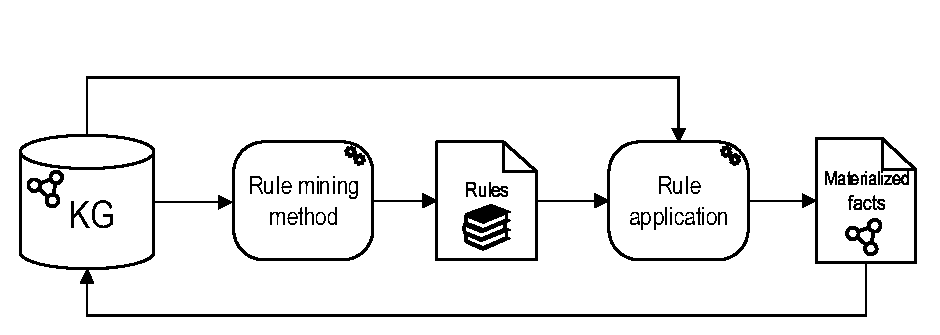
\includegraphics[width=.85\textwidth]{fig/rules/rule_process}
%     \caption{Extracting and applying rules on a Knowledge Graph}
%     \label{fig:rule-process}
% \end{figure}

% In this chapter, we present the existing methods in the literature for obtaining and applying first-order rules to complete a Knowledge Graph. First, we introduce the methods that focus solely on rule extraction. Then, we present some applications of first-order rules to the task of candidate filtering. Finally, we discuss some proposals that combine rules with other ideas presented in previous chapters.

\section{Rule mining methods}\label{sec:rule-ilp}
% There are a number of approaches to mine first-order rules in Knowledge Graphs. One of them is using Inductive Logic Programming (ILP) \cite{muggleton1994}, a classical statistical relational learning method that can be used to extract such rules from a collection of facts.

% In this regard, \citet{jiang2016} have proposed using ILP to perform Knowledge Graph completion on KGs that have a strong time constraint component. Such a KG may contain information on whether a person is the president of a country, whose correctness depends on the time period in which it is interpreted. In this proposal, the most common time periods for an assortment of different facts are inferred through ILP, and then used to assess the correctness of future facts. However, it relies on all facts having time annotations, which may not be commonplace.

% \citet{galarraga2015} proposed the AMIE+ method, which generates similar rules using ILP. AMIE+ addresses the fact that, due to the Open World Assumption (OWA), a fact that is not present in a KG should not be considered false, but instead simply unknown. The OWA thus makes it very challenging to generate truly false examples to assess the overall validity of a rule. The authors use a bespoke confidence measure for their rules, known as the partial completeness assumption confidence. AMIE+ improves the efficiency of its predecessor method AMIE \cite{galarraga2013} and can be applied to larger Knowledge Graphs.

% \citet{wang2015} refine this idea with their RDF2Rules method. Contrary to AMIE+, which is limited to only being able to mine one rule at a time, RDF2Rules speeds up the process by parallelizing rule extraction. It achieves this by detecting and extracting frequent relation cycles of a certain length in a KG, which are essentially loops that contain a given amount of relations. An example of such a loop can be found in Figure~\ref{fig:rule-cycle}. Note that the directionality of the edges in a KG is relevant for the existence of a cycle. Once the most common cycles have been obtained, a number of rules can be extracted from them. This is done by iteratively selecting one relation as the head of the rule and the rest as the body, advancing on the loop, and repeating this process until the entire loop has been traversed.

% \begin{figure}[!htp]
%     \centering
%     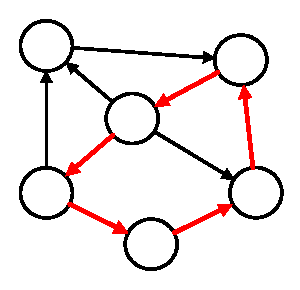
\includegraphics[width=.35\textwidth]{fig/rules/cycle}
%     \caption{A cycle of 5 relations in a sample Knowledge Graph}
%     \label{fig:rule-cycle}
% \end{figure}

% The Never-Ending Language Learning (NELL) system that was proposed by \citet{mitchell2018} also learns knowledge rules from the data that it is constantly provided. These rules are manually screened to ensure a high level of quality, so as to not introduce incorrect facts into a Knowledge Graph. It then applies these rules to generate knowledge that was previously missing.

% Markov Logic Networks (MLNs) \cite{richardson2006} have also been used for the task of completing a Knowledge Graph. MLNs combine the previously discussed rules with probabilistic models, which allows them to derive generalized knowledge from a smaller corpus of facts and to better handle complex and noisy information \cite{yang2017}.

% The use of MLNs for Knowledge Graph completion has been analyzed by \citet{kuzelka2019}. The authors conclude that MLNs can provide a satisfactory performance on this task, assuming that the triples that are missing from the graph are independent from one another and have a roughly equal probability of being true, which is not always the case \cite{borrego2019}.

% \citet{yang2017} presented Neural Logic Programming (NeuralLP), an approach that combines first-order rule mining with sparse matrix multiplication. In this approach, the authors propose using an attention mechanism to further refine the confidence value that is assigned to each individual triple. The main rule mining mechanism in NeuralLP is governed by a central neural controller. Additionally, it is able to learn rules of variable length with more ease than its predecessors.

% Furthermore, \citet{sadeghian2019} introduced DRUM, which extends NeuralLP by analyzing the structure and confidence values of the rules that are being inferred, and then approximating these elements for other rules using tensors. It, however, is only limited to positive examples due to the OWA and is not able to infer negative rules. 

% \citet{rocktaschel2017} proposed NTP, a similar method to NeuralLP, which infers rules by using transitive relations between facts. Their approach requires that such relations be represented as a vector or a tensor, in order to leverage the semantic similarities that are commonly exploited in embedded spaces. It nonetheless suffers from a lesser scalability than the original NeuralLP method, due to the computational complexity that is required to carry out the process of rule inference.

% To address the aforementioned scalability issues, \citet{minervini2018} presented an improved NTP2.0 method. This new version is able to focus only on the most promising rules during the mining process, by using a pooling method that is able to monitor the creation of multiple rules at once.

\section{Candidate filtering}\label{sec:rule-cands}
% Some authors have proposed rule-based techniques for filtering candidate triples, instead of generating new knowledge. The process of generating and applying these rules is fundamentally different: due to the very large number of possible candidate triples, the rules must not be computationally expensive to apply. Additionally, it is not as important for them to be fully correct, since an incorrect fact will be evaluated in more detail further down the KG completion process. It is, however, desirable that the candidate filtering rules exclude as few correct candidates as possible, in order not to hinder the quality of the final set of generated triples.

% \citet{wei2015} proposed the INS method, which uses the previously discussed TransE embedding model to filter out possibly incorrect knowledge. More specifically, they employ TransE to analyze the semantic similarity between the two entities in a triple, and discard the triple if the similarity does not exceed a certain threshold. This results in sets of candidate triples that are smaller than the original ones.

% \citet{shi18} also argued that it is generally not practical to apply any model to the whole set of possible candidate triples, and that it must be narrowed down in some way. In their work, they use a set of simple rules to determine that any given triple $(s, r, t)$ is a valid candidate if another triple with the structure $(\_, r, t)$ is already present in the Knowledge Graph.

% \citet{zhang2019} proposed IterE, an approach that prunes knowledge using graph traversing and random selection. It generates a set of plausible rules and monitors their performance as they are being built, removing those that are found not satisfactory and leaving only a smaller set of rules that can be generated quickly.

% Some of the previously discussed works can also be used for filtering candidate triples. The authors of NTP2.0 \cite{minervini2018} proved that a k-nearest neighbor search can provide satisfactory results to filter out wrong knowledge when inferring rules, which can be performed efficiently.

% Other proposals incorporate parameters that can be fine-tuned to rapidly rule out rules that are not satisfactory. \citet{omran2018} proposed RLvLR, which allows the user to set values for the minimum required confidence for a rule. A similar approach is followed by the already discussed DRUM \cite{sadeghian2019} method.

% Additionally, the AMIE+ method \cite{galarraga2015} can also be used for this purpose. It includes a number of strategies that can be used to prune a set of candidate triples, by producing simpler rules with a high support. Additionally, AMIE+ can perform confidence approximations, which allows it to speed up the rule inference process, making it more appealing for its application to candidate filtering.


\section{Hybrid approaches}\label{sec:rule-hybrid}
% Even though rule-based approaches excel in their explainability, they often have trouble scaling up to very large Knowledge Graphs \cite{shen2022overview}. To overcome this issue, many authors have proposed methods that combine more traditional rule mining with other approaches discussed in previous chapters, to try to guide the rule mining process towards more promising rules.

% One of the first such proposals was made by \citet{wang2015b}, who introduced the r-KGE method. It combines the tensor-based model RESCAL, the embedding-based model TransE, and logical rules. These rules are then used to prune the embedded space using integer linear programming \cite{schrijver1999}, which sees a significant reduction of its size. However, it is not properly equipped to handle N-to-N relations, and its reasoning process can still be quite computationally expensive. The overall model proposed by r-KGE is shown in Figure~\ref{fig:rule-rkge}.

% \begin{figure}[!htp]
%     \centering
%     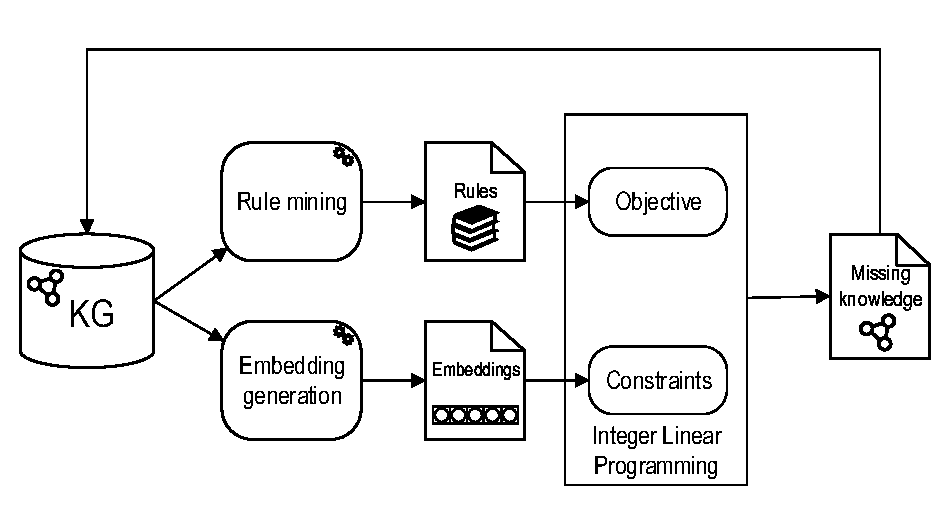
\includegraphics[width=.9\textwidth]{fig/rules/rkge}
%     \caption{Overview of the r-KGE model}
%     \label{fig:rule-rkge}
% \end{figure}

% The previously discussed INS method \cite{wei2015} also incorporates TransE to quickly compute the degree of similarity between entities, and limits the rule reasoning process by taking only the top N most similar entities into consideration. Additionally, this similarity score can provide an approximation of the quality of a rule before it is completely built.

% \citet{guo2016} introduced KALE, another model that combines logical rules and entity embeddings. KALE aims to provide a common ground in which rules and embeddings can directly interact, by representing triples as atomic formulae and rules as combination of these formulae. The semantic similarity information that is intrinsically present in the entity embeddings aids in expanding the predictive capabilities of the rules and their generality. A visual overview of the KALE architecture is provided in Figure~\ref{fig:rule-kale}. In this Figure, entity embeddings are represented in blue, relation embeddings in orange, and scalar confidence values in green.

% \begin{figure}[!htp]
%     \centering
%     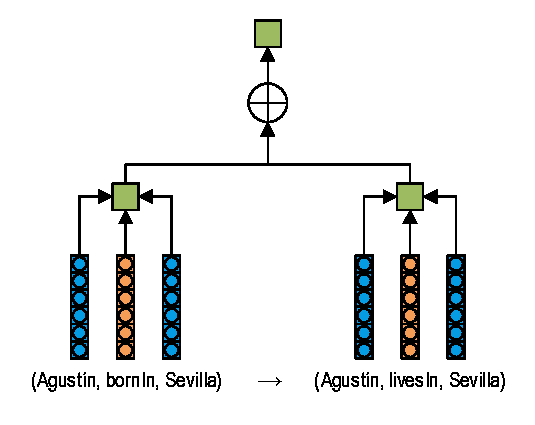
\includegraphics[width=.65\textwidth]{fig/rules/kale}
%     \caption{Overview of the KALE model}
%     \label{fig:rule-kale}
% \end{figure}

% The same authors \cite{guo2018} also presented RUGE, a KG completion technique that combines the same elements in an iterative fashion. Rather than relying on pre-computed entity embeddings, RUGE generates its own embedded space with the aid of logical rules. Additionally, RUGE is able to operate on Knowledge Graphs that has both labeled and unlabeled triples. A series of logical rules are applied on the unlabeled triples to label them. Then, the labeled triples are used to rectify and improve the embedded space so that it better captures the relations between the entities. The improved embedded space provides feedback on the labels, and the rules can be updated accordingly. A diagram depicting this process can be found in Figure~\ref{fig:rule-ruge}.

% \begin{figure}[!htp]
%     \centering
%     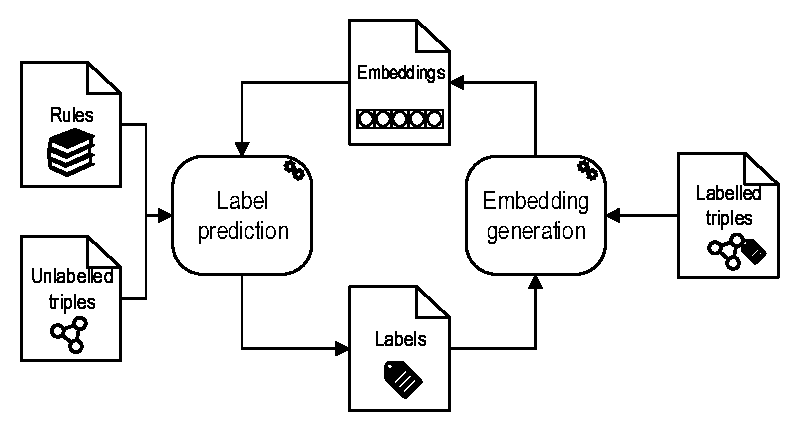
\includegraphics[width=.85\textwidth]{fig/rules/ruge}
%     \caption{Overview of the RUGE model}
%     \label{fig:rule-ruge}
% \end{figure}

% Furthermore, another aforementioned method, IterE \cite{zhang2019}, proposes a similar approach. IterE generates an initial set of entity embeddings for the Knowledge Graph. These embeddings are used to generate a set of rules, whose quality is evaluated. The best-performing rules are then used to generate new triples that are introduced in the KG, and the process starts anew by generating new embeddings that take into account the newly generated knowledge. This is shown in a graphical manner in Figure~\ref{fig:rule-itere}.

% \begin{figure}[!htp]
%     \centering
%     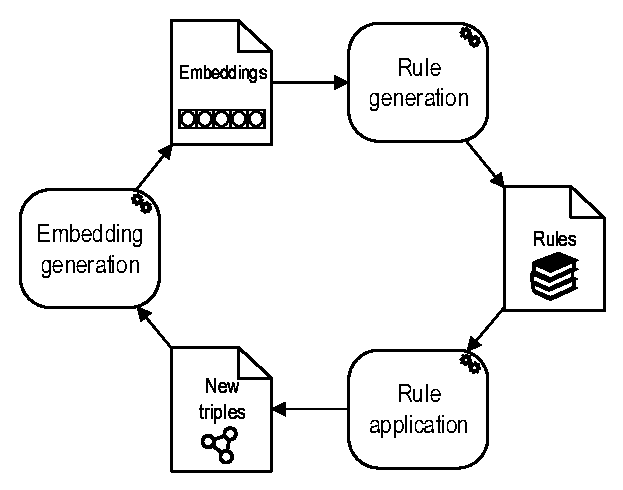
\includegraphics[width=.65\textwidth]{fig/rules/itere}
%     \caption{Overview of the IterE model}
%     \label{fig:rule-itere}
% \end{figure}

% \citet{meilicke2019} proposed AnyBURL, a technique that can generate logic rules in a bottom-up manner and on-demand. AnyBURL works by deconstructing a Knowledge Graph into a set of labeled paths. Then, it uses path-based features to determine which paths contain more useful information to obtain rules from. AnyBURL is more lightweight than other related rule-based proposals and, due to the fact that it only considers the most promising paths inside a KG, can be applied to larger graphs.

% \citet{niu2020} presented RPJE, a proposal that brings together path-based information and first-order rules. It first mines logical rules, and then uses those of length 2 to combine paths in the KG, and rules of length 1 to create a number of semantic relations.

% Finally, \citet{ma2019} introduced ELPKG, a proposal that brings together all three main approaches that we have covered in the previous chapters. It uses entity embeddings to represent the relations between entities, and a breadth-first search to detect the paths between the two entities in a triple. The information gained from both the embeddings and the paths is combined together, and it then applies soft logic to obtain the final confidence value for the triple. 

\section{Summary}\label{sec:rule-summary}
% This chapter has provided an overview of the current approaches to Knowledge Graph completion that are based on logical rules. First, we have introduced the proposals that can be found in the literature that rely solely on obtaining and applying these rules. Then, we have focused on the methods for filtering candidate triples using first-order rules. At last, we covered the methods that combine rule mining with path-based information or latent representations, such as tensors or entity embeddings.